%%%%%%%%%%%%%%%%%%%%% {{{
%%Options for presentations (in-class) and handouts (e.g. print).
\documentclass[pdf,9pt]{beamer}


%%%%%%%%%%%%%%%%%%%%%%
%Change this for different slides so it appears in bar
\usepackage{authoraftertitle}
\date{Chapter 8. Orthogonality \\ \S  8-2. Orthogonal Diagonalization}

%%%%%%%%%%%%%%%%%%%%%%
%% Upload common style file
\usepackage{LyryxLAWASlidesStyle}

\begin{document}

%%%%%%%%%%%%%%%%%%%%%%%
%% Title Page and Copyright Common to All Slides

%Title Page
\input frontmatter/titlepage.tex

%LOTS Page
\input frontmatter/lyryxopentexts.tex

%Copyright Page
\input frontmatter/copyright.tex

%%%%%%%%%%%%%%%%%%%%%%%%% }}}
%-------------- start slide -------------------------------%{{{ 2

\begin{frame}[fragile]
   \tableofcontents
\end{frame}
%-------------- end slide -------------------------------%}}}
\section[\textcolor{yellow}{}]{\textcolor{yellow}{Orthogonal Matrices}}
%-------------- start slide -----------------------------% {{{ 3
\frame{
\frametitle{Orthogonal Matrices}
\pause
\begin{definition}
  An $n\times n$ matrix $A$ is a \alert{orthogonal}
  if its inverse is equal to its transpose, i.e.,
  \alert{$A^{-1}=A^T$.}
\end{definition}
\vfill
\pause
\begin{example}
  \[ \frac{\sqrt{2}}{2}\left[\begin{array}{rr}
  1 & 1 \\ -1 & 1 \end{array}\right]
  \quad\text{and}\quad
  \frac{1}{7}\left[\begin{array}{rrr}
  2 & 6 & -3 \\ 3 & 2 & 6 \\ -6 & 3 & 2 \end{array}\right] \]
  are orthogonal matrices (verify).
\end{example}
}
%-------------- end slide -------------------------------%}}}
%-------------- start slide -----------------------------% {{{ 4
\frame{
\begin{theorem}
  The following are equivalent for an $n\times n$ matrix $A$.
  \begin{enumerate}
  \item $A$ is orthogonal.
  \item The rows of $A$ are orthonormal.
  \item The columns of $A$ are orthonormal.
  \end{enumerate}
\end{theorem}
\pause
\vfill
\begin{proofnoend}
    ``(1) $\Longleftrightarrow$ (3)": Write $A=[\vec{a}_1,\cdots \vec{a}_n]$.
    \begin{align*}
	\text{$A$ is orthogonal} & \Longleftrightarrow A^T A = I_n \Longleftrightarrow  \begin{pmatrix} \vec{a}_1^T\\ \vdots\\ \vec{a}_n \end{pmatrix} [\vec{a}_1,\cdots \vec{a}_n]= I_n\\
				 & \Longleftrightarrow
\begin{bmatrix}
    \textcolor{red}{\vec{a}_1\cdot\vec{a}_1} & \vec{a}_1\cdot\vec{a}_2                  & \cdots                  & \vec{a}_1\cdot\vec{a}_n                  \\
    \vec{a}_2\cdot\vec{a}_1                  & \textcolor{red}{\vec{a}_2\cdot\vec{a}_2} & \cdots                  & \vec{a}_2\cdot\vec{a}_n                  \\
    \vdots                                   & \vdots                                   & \textcolor{red}{\ddots} & \vdots                                   \\
    \vec{a}_n\cdot\vec{a}_1                  & \vec{a}_n\cdot\vec{a}_2                  & \cdots                  & \textcolor{red}{\vec{a}_n\cdot\vec{a}_n} \\
\end{bmatrix}
=
\begin{bmatrix}
    \textcolor{red}{1} & 0                  & \cdots                  & 0                  \\
    0                  & \textcolor{red}{1} & \ddots                  & 0                  \\
    \vdots             & \ddots             & \textcolor{red}{\ddots} & \vdots             \\
    0                  & 0                  & \cdots                  & \textcolor{red}{1} \\
\end{bmatrix}
    \end{align*}
    \bigskip

    ``(1) $\Longleftrightarrow$ (2)": Similarly (Try it yourself). \myQED
\end{proofnoend}
}
%-------------- end slide -------------------------------%}}}
% %-------------- start slide -----------------------------% {{{{ --
% \frame{
%   \begin{proofnoend}[Proof that (1) is equivalent to (3)]
%   Let $A=\left[\begin{array}{cccc}
%   \vec{x}_1 & \vec{x}_2 & \cdots & \vec{x}_n \end{array}\right]$ where
%   $\vec{x}_1,\vec{x}_2, \ldots, \vec{x}_n\in\RR^n$.
%   \pause
%   \begin{itemize}
%   \item $A$ is orthogonal if and only if $A^T=A^{-1}$.
%   \pause
%   \item  $A^T=A^{-1}$ if and only if $A^TA=I$.
%   \pause
%   \item  $A^TA=I$ if and only if
%   $\left[\begin{array}{c}
%   \vec{x}_1^T \\ \vec{x}_2^T \\ \vdots \\ \vec{x}_n^T \end{array}\right]
%   \left[\begin{array}{cccc}
%   \vec{x}_1 & \vec{x}_2 & \cdots & \vec{x}_n \end{array}\right] = I$.
%   \pause
%   \item
%   $\left[\begin{array}{c}
%   \vec{x}_1^T \\ \vec{x}_2^T \\ \vdots \\ \vec{x}_n^T \end{array}\right]
%   \left[\begin{array}{cccc}
%   \vec{x}_1 & \vec{x}_2 & \cdots & \vec{x}_n \end{array}\right] = I$
%   if and only if $\vec{x}_j\dotprod \vec{x}_j =1$ for all $j$,
%   \hspace*{.6in}$1\leq j\leq n$, and $\vec{x}_i\dotprod \vec{x}_j =0$
%   for all $i$ and $j$, $1\leq i\neq j\leq n$, i.e., the
%   \hspace*{.57in} columns of
%   $A$ are orthonormal.
%   \end{itemize}
%   \myQED\end{proofnoend}
% }
% %-------------- end slide -------------------------------%}}}
%-------------- start slide -----------------------------% {{{{ 5
\frame{
\begin{example}
  \[ A=\left[\begin{array}{rrr}
  2 & 1 & -2 \\ -2 & 1 & 2 \\ 1 & 0 & 8
  \end{array}\right]\]
  has \alert{orthogonal columns}, but its rows are not orthogonal (verify).
  \medskip

  \pause
  Normalizing the columns of $A$ gives us the matrix
  \[ A^{\prime} =\left[\begin{array}{rcr}
      2/3  & 1/{\sqrt{2}} & -1/{3\sqrt{2}} \\
      -2/3 & 1/{\sqrt{2}} & 1/{3\sqrt{2}}  \\
      1/3  & 0            & 4/{3\sqrt{2}}
  \end{array}\right],\]
  which has orthonormal columns.
  Therefore, $A^{\prime}$ is an orthogonal matrix.
\end{example}
\pause
\begin{emptytitle}
  If an $n\times n$ matrix has orthogonal rows
  (columns), then normalizing the rows (columns)
  results in an orthogonal matrix.
\end{emptytitle}
}
%-------------- end slide -------------------------------%}}}
%-------------- start slide -----------------------------% {{{{ 6
\frame{
\begin{example}[ Orthogonal Matrices: Products and Inverses ]
  Suppose $A$ and $B$ are orthogonal matrices.
  \begin{enumerate}
  \item Since
      \[ (AB)(B^TA^T)=A(BB^T)A^T =AA^T=I.\]
      and $AB$ is square, $B^TA^T=(AB)^T$ is the inverse of
      $AB$, so $AB$ is invertible, and $(AB)^{-1}=(AB)^T$.
      Therefore, \alert{$AB$ is orthogonal.}
      \pause
  \item \alert{$A^{-1}=A^T$ is also orthogonal}, since
      \[ \alert{(A^{-1})^{-1}} = A = (A^T)^{T} =\alert{(A^{-1})^{T}}.\]
  \end{enumerate}
\end{example}
\pause
\vfill
\begin{remark}[ Summary ]
  If $A$ and $B$ are orthogonal matrices, then $AB$ is orthogonal
  and $A^{-1}$ is orthogonal.
\end{remark}
}
%-------------- end slide -------------------------------%}}}
\section[\textcolor{yellow}{}]{\textcolor{yellow}{Orthogonal Diagonalization and Symmetric Matrices}}
%-------------- start slide -----------------------------% {{{{ 7
\frame{
\frametitle{Orthogonal Diagonalization and Symmetric Matrices}
\pause
\begin{definition}
  An $n\times n$ matrix $A$ is
  \alert{orthogonally diagonalizable}
  if there exists an \textcolor{blue}{orthogonal matrix, $P$,}
  so that $P^{-1}AP=P^TAP$ is diagonal.
\end{definition}
\pause
\vfill
\begin{theorem}[Principal Axis Theorem]
    Let $A$ be an $n\times n$ matrix.  The following conditions are equivalent.
    \begin{enumerate}
      \item $A$ has an orthonormal set of $n$ eigenvectors.
      \item $A$ is orthogonally diagonalizable.
      \item $A$ is symmetric.
    \end{enumerate}
\end{theorem}
}
%-------------- end slide -------------------------------%}}}
%-------------- start slide -------------------------------%{{{{ 8
\begin{frame}[fragile]
  \begin{proofnoend}[ (1) $\Rightarrow$ (2)]
    Suppose $\{ \vec{x}_1, \vec{x}_2, \ldots, \vec{x}_n\}$ is
    an orthonormal set of $n$ eigenvectors of $A$.
    Then $\{ \vec{x}_1, \vec{x}_2, \ldots, \vec{x}_n\}$ is
    a basis of $\RR^n$, and hence
    $P=\left[\begin{array}{cccc}
    \vec{x}_1 & \vec{x}_2 & \cdots &\vec{x}_n\end{array}\right]$
    is an orthogonal matrix such that $P^{-1}AP=P^TAP$ is a diagonal matrix.
    Therefore $A$ is orthogonally diagonalizable.
\end{proofnoend}
\end{frame}
%-------------- end slide -------------------------------%}}}
%-------------- start slide -----------------------------% {{{{ 9
\frame{
\begin{proofnoend}[ (2) $\Rightarrow$ (1)]
  Suppose that $A$ is orthogonally diagonalizable.
  Then there exists an orthogonal matrix $P$ such that
  $P^TAP$ is a diagonal matrix.
  If $P$ has columns $\vec{x}_1, \vec{x}_2, \ldots, \vec{x}_n$,
  then $B=\{ \vec{x}_1, \vec{x}_2, \ldots, \vec{x}_n\}$ is
  a set of $n$ orthonormal vectors in $\RR^n$.
  Since $B$ is orthogonal, $B$ is independent;
  furthermore, since $|B|=n=\dim(\RR^n)$, $B$ spans $\RR^n$
  and is therefore a basis of $\RR^n$.

  Let $P^TAP=\diag(\ell_1, \ell_2, \ldots, \ell_n)=D$.
  Then $AP=PD$, so
  \begin{eqnarray*}
      A\left[\begin{array}{cccc}
      \vec{x_1} & \vec{x_2} & \cdots & \vec{x_n}
      \end{array}\right]
      & = &
      \left[\begin{array}{cccc}
      \vec{x_1} & \vec{x_2} & \cdots & \vec{x_n} \end{array}\right]
      \left[\begin{array}{cccc}
          \ell_1 & 0      & \cdots & 0      \\
          0      & \ell_2 & \cdots & 0      \\
          \vdots & \vdots &        & \vdots \\
          0      & 0      & \cdots & \ell_n
      \end{array}\right]\\
      \left[\begin{array}{cccc}
      A\vec{x_1} & A\vec{x_2} & \cdots & A\vec{x_n} \end{array}\right]
      & = & \left[\begin{array}{cccc}
      \ell_1\vec{x_1} & \ell_2\vec{x_2} & \cdots & \ell_n\vec{x_n}
      \end{array}\right]
  \end{eqnarray*}

  Thus $A\vec{x}_i=\ell_i\vec{x}_i$ for each $i$, $1\leq i\leq n$,
  implying that $B$ consists of eigenvectors of $A$.
  Therefore, $A$ has an orthonormal set of $n$ eigenvectors.
\end{proofnoend}
}
%-------------- end slide -------------------------------%}}}
%-------------- start slide -----------------------------% {{{ 10
\frame{
\begin{proofnoend}[(2) $\Rightarrow$ (3)]
  Suppose $A$ is orthogonally diagonalizable, that $D$ is
  a diagonal matrix, and that $P$ is
  an orthogonal matrix so that $P^{-1}AP=D$.
  \pause
  Then $P^{-1}AP=P^TAP$, so
  \[ A=PDP^T.\]
  \pause
  Taking transposes of both sides of the equation:
  \begin{eqnarray*}
      A^T=(PDP^T)^T
      & = & (P^T)^T D^T P^T \\
      & = & P D^T P^T \alert{\mbox{~~(since } (P^T)^T=P)} \\
      & = & P D P^T \hspace*{.2in}\alert{\mbox{(since } D^T=D)} \\
      & = & A.
  \end{eqnarray*}
  \pause
  Since $A^T=A$, $A$ is symmetric.
\end{proofnoend}
}
%-------------- end slide -------------------------------%}}}
%-------------- start slide -----------------------------% {{{ 11
\frame{
\begin{proofnoend}[(3) $\Rightarrow$ (2)]
  If $A$ is $n\times n$ symmetric matrix, we will prove by induction on $n$
  that $A$ is orthogonal diagonalizable.  If $n=1$, $A$ is already
  diagonalizable. If $n\ge 2$, assume that (3)$\Rightarrow$(2) for all
  $(n-1)\times(n-1)$ symmetric matrix.
  \bigskip

  First we know that all eigenvalues are real (because $A$ is symmetric). Let $\lambda_1$ be one
  real eigenvalue and $\vec{x}_1$ be the normalized eigenvector. We can extend $\{\vec{x}_1\}$ to an
  orthonormal basis of $\R^n$, say $\{\vec{x}_1,\cdots, \vec{x}_n\}$ by adding vectors. Let
  $P_1=[\vec{x}_1,\cdots,\vec{x}_n]$. So $P$ is orthogonal.

  Now we can apply the technical lemma proved in Section 5.5 to see that
  \begin{align*}
      P_1^T AP_1 = \begin{bmatrix} \lambda_1 & B \\ \vec{0} & A_1  \end{bmatrix}.
  \end{align*}
  Since LHS is symmetric, so does the RHS. This implies that $B=O$ and $A_1$ is symmetric.
\end{proofnoend}
}
%-------------- end slide -------------------------------%}}}
%-------------- start slide -----------------------------% {{{ 12
\frame{
\begin{proofnoend}[(3) $\Rightarrow$ (2) -- continued]
    By induction assumption, $A_1$ is orthogonal diagonalizable, i.e., for some orthogonal matrix $Q$
    and diagonal matrix $D$, $A_1 = QDQ^T$. Hence,
    \begin{align*}
      P_1^T AP_1  = \begin{bmatrix} \lambda_1 & \vec{0}^T \\ \vec{0} & QDQ^T  \end{bmatrix}
		  =  \begin{bmatrix} 1 & \vec{0}^T \\ \vec{0} & Q  \end{bmatrix}
	    \begin{bmatrix} \lambda_1 & \vec{0}^T \\ \vec{0} & D  \end{bmatrix}
	    \begin{bmatrix} 1 & \vec{0}^T \\ \vec{0} & Q^T  \end{bmatrix}
    \end{align*}
    which is nothing but
    \begin{align*}
      A  & = P_1\begin{bmatrix} 1 & \vec{0}^T \\ \vec{0} & Q  \end{bmatrix}
	    \begin{bmatrix} \lambda_1 & \vec{0}^T \\ \vec{0} & D  \end{bmatrix}
	    \begin{bmatrix} 1 & \vec{0}^T \\ \vec{0} & Q^T  \end{bmatrix} P_1^T\\
	& = \left(P_1\begin{bmatrix} 1 & \vec{0}^T \\ \vec{0} & Q  \end{bmatrix}\right)
	    \begin{bmatrix} \lambda_1 & \vec{0}^T \\ \vec{0} & D  \end{bmatrix}
	    \left(P_1\begin{bmatrix} 1 & \vec{0}^T \\ \vec{0} & Q  \end{bmatrix} \right)^T.
    \end{align*}

    \bigskip
    Finally, it is ready to verify that the matrix
    \begin{align*}
	P_1\begin{bmatrix} 1 & \vec{0}^T \\ \vec{0} & Q  \end{bmatrix}
    \end{align*}
    is a diagonal matrix. This complete the proof of the theorem.
    \myQED
\end{proofnoend}
}
%-------------- end slide -------------------------------%}}}
%-------------- start slide -----------------------------% {{{ 13
\frame{
\begin{definition}
  Let $A$ be an $n\times n$ matrix.
  A set of $n$ orthonormal eigenvectors of $A$ is called
  a set of \alert{principal axes} of $A$.
\end{definition}
}
%-------------- end slide -------------------------------%}}}
%-------------- start slide -----------------------------% {{{ 14
\frame{
\begin{problem}
  %Find an orthogonal matrix $P$ such that
  %$P^TAP$ is diagonal, where
  Orthogonally diagonalize the matrix
  \[ A=\left[\begin{array}{rrr}
  1 & -2 & -2 \\ -2 & 1 & -2 \\ -2 & -2 & 1
  \end{array}\right].\]
\end{problem}
\pause
\begin{solution}
  \begin{itemize}
  \item $c_A(x)=(x+3)(x-3)^2$, so $A$ has eigenvalues
  $\lambda_1=3$ of multiplicity two, and
  $\lambda_2=-3$.
  \pause
  \item $\{ \vec{x}_1, \vec{x}_2\}$ is a basis of $E_3(A)$, where
  $\vec{x}_1 = \left[ \begin{array}{r} -1 \\ 0 \\ 1 \end{array}\right]$
  and
  $\vec{x}_2 = \left[ \begin{array}{r} -1 \\ 1 \\ 0\end{array}\right]$.
  \pause
  \item $\{ \vec{x}_3\}$ is a basis of $E_{-3}(A)$, where
  $\vec{x}_3 = \left[ \begin{array}{r} 1 \\ 1 \\ 1 \end{array}\right]$.
  \pause
  \item $\{ \vec{x}_1, \vec{x}_2, \vec{x}_3 \}$ a linearly
  independent set of eigenvectors of $A$, and a basis of $\RR^3$.
  \end{itemize}
\end{solution}
}
%-------------- end slide -------------------------------%}}}
%-------------- start slide -----------------------------% {{{ 15
\frame{
\begin{solution}[continued]
\begin{itemize}
    \item Orthogonalize $\{ \vec{x}_1, \vec{x}_2, \vec{x}_3 \}$ using the Gram-Schmidt orthogonalization algorithm.
	\pause
	\item Let
	$\vec{f_1} = \left[ \begin{array}{r} -1 \\ 0 \\ 1  \end{array}\right],
	 \vec{f_2} = \left[ \begin{array}{r} -1 \\ 2 \\ -1 \end{array}\right]$ and
	$\vec{f_3} = \left[ \begin{array}{r} 1  \\ 1 \\ 1  \end{array}\right]$.
	Then
	$\{ \vec{f_1}, \vec{f_2}, \vec{f_3} \}$ is an orthogonal basis
	of $\RR^3$ consisting of eigenvectors of $A$.
	\pause
    \item Since $||\vec{f_1} ||=\sqrt{2}$,
	$||\vec{f_2} ||=\sqrt{6}$, and $||\vec{f_3} ||=\sqrt{3}$,
	\[ P= \left[\begin{array}{ccc}
	-1/\sqrt{2} & -1/\sqrt{6} & 1/\sqrt{3} \\
	0 & 2/\sqrt{6} & 1/\sqrt{3} \\
	1/\sqrt{2} & -1/\sqrt{6} & 1/\sqrt{3}
	\end{array}\right] \]
	is an orthogonal diagonalizing matrix of $A$,
	\pause
	and
	\[ P^TAP=\left[\begin{array}{ccc}
	    3 & 0 & 0 \\
	    0 & 3 & 0 \\
	    0 & 0 & -3
	\end{array}\right]. \]
\end{itemize}
\myQED
\end{solution}
}
%-------------- end slide -------------------------------%}}}
%-------------- start slide -----------------------------% {{{ 16
\frame{
\begin{theorem}
  If $A$ is a symmetric matrix, then the eigenvectors of $A$
  corresponding to distinct eigenvalues are orthogonal.
\end{theorem}
\pause
\vfill
\begin{proofnoend}
  Suppose $\lambda$ and $\mu$ are eigenvalues of $A$, $\lambda\neq \mu$,
  and let $\vec{x}$ and $\vec{y}$, respectively, be corresponding
  eigenvectors,
  i.e., \alert{$A\vec{x}=\lambda\vec{x}$ and $A\vec{y}=\mu\vec{y}$.}
  Consider $(\lambda-\mu)\vec{x}\dotprod\vec{y}$.
  \pause
  \begin{eqnarray*}
      (\lambda-\mu)\vec{x}\dotprod\vec{y}
      & = & \lambda(\vec{x}\dotprod\vec{y}) -\mu(\vec{x}\dotprod\vec{y}) \\ \pause
      & = & (\lambda\vec{x})\dotprod\vec{y} -\vec{x}\dotprod(\mu\vec{y}) \\ \pause
      & = & (A\vec{x})\dotprod\vec{y} -\vec{x}\dotprod(A\vec{y}) \\ \pause
      & = & (A\vec{x})^T\vec{y} -\vec{x}^T(A\vec{y}) \\ \pause
      & = & \vec{x}^TA^T\vec{y} -\vec{x}^TA\vec{y} \\ \pause
      & = & \vec{x}^TA\vec{y} -\vec{x}^TA\vec{y} \hspace*{.3in}{\mbox{ since $A$ is symmetric}} \\ \pause
      & = & 0.
  \end{eqnarray*}
  % \vspace*{-.2in}

  \pause
  Since $\lambda\neq \mu$, $\lambda- \mu\neq 0$,
  and therefore $\vec{x}\dotprod\vec{y}=0$,
  i.e., $\vec{x}$ and $\vec{y}$ are orthogonal.
  \myQED
\end{proofnoend}
}
%-------------- end slide -------------------------------%}}}
%-------------- start slide -----------------------------% {{{ 17
\frame{
\begin{remark}[ Diagonalizing a Symmetric Matrix ]
    Let $A$ be a symmetric $n\times n$ matrix.
    \begin{enumerate}
      \item Find the characteristic polynomial and distinct eigenvalues of $A$.
      \item For each distinct eigenvalue $\lambda$ of $A$, find an
	  \alert{orthonormal basis} of $E_A(\lambda)$, the eigenspace
	  of $A$ corresponding to $\lambda$.
	  This requires using the Gram-Schmidt orthogonalization
	  algorithm when $\dim(E_A(\lambda))\ge 2$.
      \item By the previous theorem, the eigenvectors of distinct
	  eigenvalues produce orthogonal eigenvectors, so the result
	  is an orthonormal basis of $\RR^n$.
    \end{enumerate}
\end{remark}
}
%-------------- end slide -------------------------------%}}}
%-------------- start slide -------------------------------%{{{ 18
\begin{frame}[fragile]
    \begin{problem}
  Orthogonally diagonalize the matrix
  \[ A=\left[\begin{array}{rrr}
      3 & 1 & 1 \\
      1 & 2 & 2 \\
      1 & 2 & 2
  \end{array}\right].\]
\end{problem}
\vfill
\pause
\begin{solution}
    \begin{enumerate}
	\item Since row sum is $5$, $\lambda_1=5$ is one eigenvalue, corresponding
	    eigenvector should be $(1,1,1)^T$. After normalization it should be
	    \begin{align*}
		\vec{v}_1=
		\begin{pmatrix}
		   \frac{1}{\sqrt{3}}\\
		   \frac{1}{\sqrt{3}}\\
		   \frac{1}{\sqrt{3}}
		\end{pmatrix}
	    \end{align*}
    \end{enumerate}
\end{solution}
\end{frame}
%-------------- end slide -------------------------------%}}}
%-------------- start slide -------------------------------%{{{ 19
\begin{frame}[fragile]
    \begin{solution}[continued]
   \begin{enumerate}
       \item[2.] Since last two rows are identical, $\det(A)=0$, so $\lambda_2=0$
	   is another eigenvalue, corresponding eigenvector should be
	   $(0,1,-1)^T$. After normalization it should be
	   \begin{align*}
	       \vec{v}_2 =
		\begin{pmatrix}
        0 		  \\
        \frac{1}{\sqrt{2}}\\
        \frac{1}{\sqrt{2}}
		\end{pmatrix}
	   \end{align*}
   \end{enumerate}
   \end{solution}
\end{frame}
%-------------- end slide -------------------------------%}}}
%-------------- start slide -------------------------------%{{{ 20
\begin{frame}[fragile]
    \begin{solution}[continued]
   \begin{enumerate}
       \item[3.] Since $\trace(A)=7 = \lambda_1+\lambda_2+\lambda_3$, we see
	   that $\lambda_3 = 7-5-0=2$. Its eigenvector should be orthogonal to
	   both $\vec{v}_1$ and $\vec{v}_2$, hence,
	   $\vec{v}_3 = (2,-1,-1)$. After normalization,
	   \begin{align*}
	    \begin{pmatrix}
        \frac{2}{\sqrt{6}} \\
        -\frac{1}{\sqrt{2}} \\
        -\frac{1}{\sqrt{2}}
	    \end{pmatrix}
	   \end{align*}
   \end{enumerate}
   \bigskip
   \pause
   Hence, we have
   \begin{align*}
      \left[\begin{array}{rrr}
        3 & 1 & 1 \\
        1 & 2 & 2 \\
        1 & 2 & 2
      \end{array}\right]
      =
    \begin{bmatrix}
      0 		   & \frac{2}{\sqrt{6}}  & \frac{1}{\sqrt{3}}\\
      \frac{1}{\sqrt{2}} & -\frac{1}{\sqrt{2}} & \frac{1}{\sqrt{3}}\\
      \frac{1}{\sqrt{2}} & -\frac{1}{\sqrt{2}} & \frac{1}{\sqrt{3}}\\
    \end{bmatrix}
    \begin{bmatrix}
      0 & 0 & 0\\
      0 & 2 & 0\\
      0 & 0 & 5\\
    \end{bmatrix}
    \begin{bmatrix}
      0                  & \frac{1}{\sqrt{2}}  & \frac{1}{\sqrt{2}}  \\
      \frac{2}{\sqrt{6}} & -\frac{1}{\sqrt{2}} & -\frac{1}{\sqrt{2}} \\
      \frac{1}{\sqrt{3}} & \frac{1}{\sqrt{3}}  & \frac{1}{\sqrt{3}}  \\
    \end{bmatrix}
   \end{align*}
   \myQED
   \end{solution}
\end{frame}
%-------------- end slide -------------------------------%}}}
\section[\textcolor{yellow}{}]{\textcolor{yellow}{Quadratic Forms}}
%-------------- start slide -----------------------------% {{{ 21
\frame{
\frametitle{Quadratic Forms}
\pause
\begin{definitions}
  Let $q$ be a real polynomial in variables $x_1$ and $x_2$ such that
  \[ q(x_1,x_2)=ax_1^2+bx_1x_2+cx_2^2.\]
  Then $q$
  is called a \alert{quadratic form} in variables $x_1$ and $x_2$.
  The term $bx_1x_2$ is called the \alert{cross term}.
  The graph of the equation $q(x_1,x_2)=1$,
  is call a \alert{conic} in variables $x_1$ and $x_2$.
\end{definitions}
}
%-------------- end slide -------------------------------%}}}
%-------------- start slide -----------------------------% {{{ 22
\frame{
\begin{example}
  % \textcolor{titletextcolour}{Example}\\[0.5em]
  Below is the graph of the equation $x_1x_2=1$.

  \begin{picture}(4,1.5)
  \put(0.5,0.2){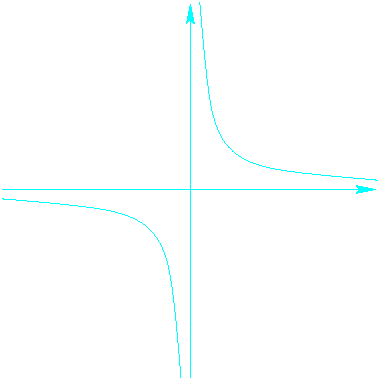
\includegraphics[scale=0.5]{figures/quadratic-1_copy.pdf}}
  \put(1.03,0.73){\scriptsize $0$}
  \put(1.3,0.65){\scriptsize $x_1x_2=1$}
  \put(1.8,0.82){\scriptsize $x_1$}
  \put(1,1.4){\scriptsize $x_2$}
  \uncover<3->{
  \put(2.5,0.2){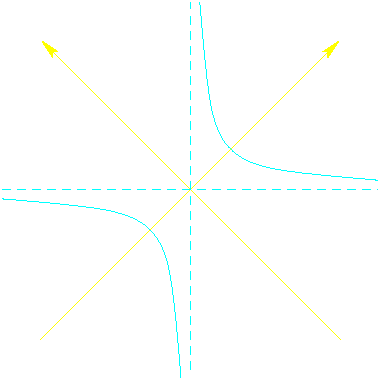
\includegraphics[scale=0.5]{figures/quadratic-2_copy.pdf}}
  \put(3.05,0.68){\scriptsize $0$}
  \put(3.4,0.65){\textcolor{yellow}{\scriptsize $y_1^2-y_2^2=1$}}
  \put(3.6,1.17){\textcolor{yellow}{\footnotesize $y_1$}}
  \put(2.6,1.17){\textcolor{yellow}{\footnotesize $y_2$}}
  \put(3.8,0.82){\scriptsize $x_1$}
  \put(3,1.4){\scriptsize $x_2$}}
  \end{picture}
  \pause

  Let $y_1$ and $y_2$ be new variables such that
  \[ x_1=y_1+y_2~\quad\text{and}\quad~ x_2=y_1-y_2,\]
  i.e., $y_1=\frac{x_1+x_2}{2}$ and $y_2=\frac{x_1-x_2}{2}$.
  Then $x_1x_2=y_1^2-y_2^2$, and $y_1^2-y_2^2$
  \uncover<2->{
  is a quadratic form with no cross terms, called a
  \alert{diagonal quadratic form};}
  \uncover<3->{
  \alert{$y_1$ and $y_2$} are called
  \alert{principal axes} of the quadratic form $x_1x_2$.
\end{example}
}}
%-------------- end slide -------------------------------%}}}
%-------------- start slide -----------------------------% {{{ 23
\frame{
\begin{emptytitle}
  Principal axes of a quadratic form can be found by using
  \alert{orthogonal diagonalization}.
\end{emptytitle}
\pause
\begin{problem}
  Find principal axes of the quadratic form
  $q(x_1,x_2)=x_1^2+6x_1x_2+x_2^2$,
  and transform $q(x_1,x_2)$ into a diagonal quadratic form.
\end{problem}
\pause
\begin{solution}
  Express $q(x_1,x_2)$ as a matrix product:
  % \vspace*{-.1in}

  \begin{equation}
      q(x_1,x_2)=
      \left[\begin{array}{cc} x_1 &  x_2 \end{array}\right]
      \left[\begin{array}{cc} 1   &  6\\ 0 & 1 \end{array}\right]
      \left[\begin{array}{c}  x_1 \\ x_2 \end{array}\right].
  \end{equation}
  % \vspace*{-.1in}

  We want a $2\times 2$ \alert{symmetric} matrix.
  Since $6x_1x_2 = 3x_1x_2 + 3x_2x_1$, we can rewrite (1) as
  % \vspace*{-.1in}

  \begin{equation}
  q(x_1,x_2)=\left[\begin{array}{cc} x_1 & x_2 \end{array}\right]
  \left[\begin{array}{cc} 1 & 3\\ 3 & 1 \end{array}\right]
  \left[\begin{array}{c} x_1 \\ x_2 \end{array}\right].
  \end{equation}
  % \vspace*{-.1in}

  Setting $\vec{x}=\left[\begin{array}{c} x_1 \\ x_2 \end{array}\right]$
  and $A=\left[\begin{array}{cc} 1 & 3\\ 3 & 1 \end{array}\right]$,
  $q(x_1,x_2)=\vec{x}^TA\vec{x}$.

  We now orthogonally diagonalize $A$.
\end{solution}
}
%-------------- end slide -------------------------------%}}}
%-------------- start slide -----------------------------% {{{ 24
\frame{
\begin{solution}[continued]
  \[c_A(z)=\left|\begin{array}{cc} z-1 & -3 \\ -3 & z-1 \end{array}\right| = (z-4)(z+2),  \]
  so $A$ has eigenvalues $\lambda_1=4$ and $\lambda_2=-2$.
  % \vspace*{-.1in}
  \pause

  \[ \vec{z}_1=\left[\begin{array}{c} 1 \\ 1 \end{array}\right]
  ~\quad\text{and}\quad~
  \vec{z}_2=\left[\begin{array}{r} -1 \\ 1 \end{array}\right] \]
  % \vspace*{-.1in}

  are eigenvectors corresponding to $\lambda_1=4$ and $\lambda_2=-2$,
  respectively.
  Normalizing these eigenvectors gives us the orthogonal matrix
  % \vspace*{-.1in}

  \[ P=\frac{1}{\sqrt{2}}
  \left[\begin{array}{cc} 1 & -1\\ 1 & 1 \end{array}\right]
  ~\mbox{ such that }~
  P^TAP=\left[\begin{array}{cc} 4 & 0\\ 0 & -2 \end{array}\right]=D. \]
  % \vspace*{-.1in}
  \pause

  Thus $A=PDP^T$, and
  \[
      q(x_1,x_2) = \vec{x}^TA\vec{x}
                 = \vec{x}^T(PDP^T)\vec{x}
                 = (\vec{x}^TP)D(P^T\vec{x})
                 = (P^T\vec{x})^TD(P^T\vec{x}).
  \]
\end{solution}
}
%-------------- end slide -------------------------------%}}}
%-------------- start slide -----------------------------% {{{ 25
\frame{
\begin{solution}[continued]
    Let
    \begin{align*}
      \vec{y} = \left[\begin{array}{c} y_1 \\ y_2 \end{array}\right]
              = P^T\vec{x}
              = \frac{1}{\sqrt{2}} \left[\begin{array}{cc} 1 & 1\\ -1 & 1 \end{array}\right] \left[\begin{array}{c} x_1 \\ x_2 \end{array}\right]
              = \frac{1}{\sqrt{2}} \left[\begin{array}{c} x_1+x_2 \\ x_2-x_1 \end{array}\right].
    \end{align*}
    Then
    \[
      q(y_1,y_2)=\vec{y}^TD\vec{y}
      = \left[\begin{array}{cc} y_1 & y_2 \end{array}\right]
      \left[\begin{array}{cc} 4 & 0\\ 0 & -2 \end{array}\right]
      \left[\begin{array}{c} y_1 \\ y_2 \end{array}\right]
      = 4y_1^2 - 2y_2^2.
    \]
    \bigskip
    \pause
    Therefore, the principal axes of $q(x_1,x_2)=x_1^2+6x_1x_2+x_2^2$ are
    \[ y_1 = \frac{1}{\sqrt{2}}(x_1 + x_2)\]
    and
    \[ y_2 = \frac{1}{\sqrt{2}}(x_2 - x_1),\]
    yielding the diagonal quadratic form
    \[ q(y_1,y_2)=4y_1^2 - 2y_2^2.\]
    \myQED
\end{solution}
}
%-------------- end slide -------------------------------%}}}
%-------------- start slide -----------------------------% {{{ 26
\frame{
\begin{problem}
  Find principal axes of the quadratic form
  \[ q(x_1,x_2)= 7x_1^2 - 4x_1x_2+4x_2^2,\]
  and transform $q(x_1,x_2)$ into a diagonal quadratic form.
\end{problem}
\vfill
\pause
\begin{solution}[ Final Answer ]
  $q(x_1,x_2)$ has principal axes
  \begin{eqnarray*}
      y_1 & = & \frac{1}{\sqrt{5}}(-2x_1+x_2), \\
      y_2 & = & \frac{1}{\sqrt{5}}(x_1+2x_2).
  \end{eqnarray*}
  yielding the diagonal quadratic form
  \[ q(y_1,y_2)=8y_1^2+3y_2^2.\]
\end{solution}
}
%-------------- end slide -------------------------------%}}}
%-------------- start slide -----------------------------% {{{ 27
\frame{
\begin{theorem}[Triangulation Theorem -- {\it Schur} Decomposition]
    Let $A$ be an $n\times n$ matrix \textcolor{yellow}{with $n$ real eigenvalues}.
    Then there exists an orthogonal matrix $P$ such that
    $P^TAP$ is \alert{upper triangular}.
\end{theorem}
}
%-------------- end slide -------------------------------%}}}
%-------------- start slide -------------------------------%{{{ 28
\begin{frame}[fragile]
\begin{corollary}
  Let $A$ be an $n\times n$ matrix with real eigenvalues
  $\lambda_1, \lambda_2, \ldots, \lambda_n$, not necessarily
  distinct.
  Then $\det(A)=\lambda_1 \lambda_2 \cdots \lambda_n$
  and $\trace(A)=\lambda_1 + \lambda_2 + \cdots + \lambda_n$.
\end{corollary}
\pause
\vfill
\begin{proofnoend}
  By the theorem, there exists an orthogonal matrix $P$ such
  that $P^TAP=U$, where $U$ is an upper triangular matrix.
  Since $P$ is orthogonal, $P^T=P^{-1}$, so $U$ is similar to $A$;
  thus the eigenvalues
  of $U$ are $\lambda_1, \lambda_2, \ldots, \lambda_n$.
  Furthermore, since $U$ is (upper) triangular, the entries on the
  main diagonal of $U$ are its eigenvalues, so
  $\det(U)=\lambda_1 \lambda_2 \cdots \lambda_n$ and
  $\trace(U)=\lambda_1 + \lambda_2 + \cdots + \lambda_n$.
  Since $U$ and $A$ are similar, $\det(A)=\det(U)$ and $\trace(A)=\trace(U)$,
  and the result follow.
  \myQED
\end{proofnoend}
\end{frame}
%-------------- end slide -------------------------------%}}}
\end{document}
